% !TEX root = ../thesis_main.tex
\chapter{Theory}\label{chap:theory}
    This chapter will provide a basis for understanding the principles on which this work is based as well as the phenomena used in the different builds. It will cover many aspects, but of course, a deeper understanding can be gained by also consulting the references mentioned.
    \section{Nuclei and Spins}
    The postulation of an electron spin in 1926 \ref{} and later, in 1928, of a proton spin \ref{} opened
    up new areas of research.\todo{more history}
    Each particle has magnetic properties to which both electrons and the nucleus, i.e. protons and neutrons, conribute. We consider the electons' contributions to be of a static nature because of the fast movement (see \ref{chemical shif, kann man so sagen?}) and instead turn to the nucleus' magnetic properties. As we want to manipulate nuclei electromagnetically, their magnetic momentum is the relevant physical property in this case.
    The magnetic momentum $\vec M$ of a nucleus is connected to the spin $\vec S$ by the gyromagnetic ratio $\gamma$, a nucleus specific proportionality factor:
    \begin{equation}
        \vec M = \gamma \vec S
        \label{eq:gyromagneticRatio}
    \end{equation}
    The spin can be described as and seems to behave like an angular momentum, but is not created by a particle rotation but rather an inrinsic property of the particle. Each of the nuclei, in case of the hydrogen nucleus also simply called "spin" as it is only a single proton and thus a single spin, is described by the quantum numbers according to the quantized angular momenta, using quantum numbers I and m. We consider the protons and neutrons to be in their spin $\tfrac{1}{2}$ state in all cases considered here, only at very high energies in the \SI{}{\giga\electronvolt}, other states can occur. The quantum numbers are described by the quantum operators   The nucleus thus has m~=~(2I~+~1) energy eigenstates that are degenerated in zero field. If a magnetic field is present though, the energy levels will split with energy differences proportional to the magnetic field strength, the Zeeman energy splittings.
    \subsection{Zeeman energy splitting}
    If a particle with a spin $S\neq 0$ is exposed to a magnetic field $B_0$, it experiences an energy splitting of its eigenstates due to the fact that the direction of the spins compared to the field is now a relevant parameter for the overall energy of the particle. Both the gyromagnetic ratio and the field strength determine how big that splitting is:
    \begin{equation}
        E_{Z} = -\gamma m B
    \end{equation}
    where $E_Z$ is the zeeman energy difference to the non-split state and m is the magnetic quantum number. The negative sign implies that a antiparallel orientation with the field for particle with positive $\gamma$ is energetically favorable. For example, $^1$H and $^{15}$N, the two main nuclei considered in this work, show energy splittings into two levels ($2\cdot\tfrac{1}{2}+1$), but of about a factor of 10 stronger for $^1$H due to the by that factor larger gyromagnetic ratio. (see figure \ref{}).
    \begin{figure}
        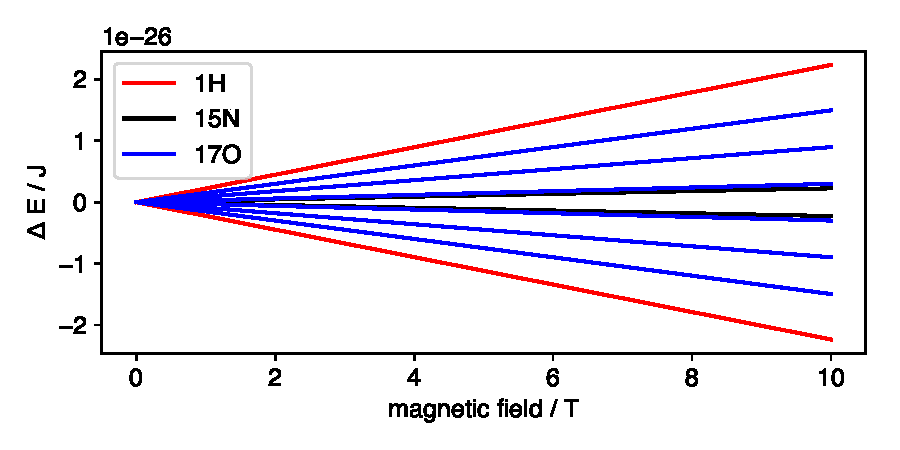
\includegraphics[width=0.99\textwidth]{/figures/theory/zeemanPlot.pdf}
        \caption[Zeeman energy splitting]{The Zeeman energy splittings of three nuclei over magnetic field. Note the difference in slopes for the spin $\tfrac{1}{2}$ nuclei 1H and 15N caused by the different gyromagnetic ratios. Arbitraily, 17O, a spin $\tfrac{5}{2}$ nucleus, was plotted to visualize higher order splittings with $2 \cdot\tfrac{5}{2}+1 = 6$ energy levels. }
    \end{figure}
    Individual spins can be described by their angular momentum operators $\hat{I}$,
    $\hat{I}_y$ and $\hat{I}_z$ that return the eigenvalue of the state in its respective
    direction.
    \begin{equation}
        \hat I_z \ket{I, S} = S \ket{I,S}
    \end{equation}
    Considering a spin-1/2 particle in a magnetic field along the z-axis (e.g. the proton as a prominent particle in NMR), these
    eigenstates are
    \begin{equation}
    \ket\alpha = \begin{pmatrix}1\\0\end{pmatrix} \hspace{2 cm} \ket\beta =
    \begin{pmatrix}0\\1\end{pmatrix}
    \end{equation}
    with the eigenvalues of $\pm 1/2$.
    Generally, every spin-1/2 particle can be in any superposition of those two eigenstates:
    \begin{equation}
        \ket\psi = c_\alpha \ket\alpha + c_\beta \ket \beta = \begin{pmatrix} c_\alpha \\
        c_\beta\end{pmatrix}
    \end{equation}
    These superposition states evolve under external conditions until a eigenstate of the particle
    is reached.
    Generally, a sample does not consist of one, but of many nuclei and thus many spins need to be
    described to describe the system. To do so, usually the density matrix formalism is introduced.
    It onsiders an ensembe of spins that do not interact with each other. In this case, the
    expectation value of an operator for a single spin $\braket{\hat Q}$ is given by
    \begin{equation}
    \bra\psi\hat Q\ket\psi = \left( c_\alpha^*, c_\beta^*\right)
    \begin{pmatrix}
        Q_{\alpha\alpha} Q_{\alpha\beta}\\
        Q_{\beta\alpha} Q_{\beta\beta}
    \end{pmatrix}
    \begin{pmatrix}
        c_\alpha\\
        c_\beta
    \end{pmatrix}
    \end{equation}
    It can be shown that this is equal to the trace of the density operator
    $\ket\psi\bra\psi$multiplied with said operator
    \begin{equation}
        \braket{\hat Q} = \Tr \left\{\ket\psi\bra\psi\hat Q\right\}
    \end{equation}
    For multiple spins, it follows that the observable becomes the sum of their individual
    observables:
    \begin{equation}
        \braket{\hat Q_{all}}= \bra{\psi_1}\hat Q\ket{\psi_1} + \bra{\psi_2}\hat Q\ket{\psi_2} + \hdots =
        \Tr{\left\{\left(\ket{\psi_1}\bra{\psi_1} + \bra{\psi_2}\ket{\psi_2}+ \hdots \right) \hat Q\right\}}
    \end{equation}
    This means that the system of spins can be described by the sum of the density operators called
    the density matrix
    \begin{equation}
        \hat\rho = \overline{\ket\psi\bra\psi}.
    \end{equation}
    For a spin-1/2 ensemble, the density matrix in thermal equilibrium is
    \begin{equation}
        \hat \rho = \begin{pmatrix} \frac{1}{2}+\frac{1}{4}\mathbb{B}& 0\\ 0&
        \frac{1}{2}-\frac{1}{4}\mathbb{B}\end{pmatrix} = \frac {1}{2} \hat1 + \frac{1}{2} \mathbb{B}
        \hat I_z
    \end{equation}
    with $\mathbb{B} = \frac{\hbar\gamma B_0}{k_b T}$. That means that in thermal equilibrium, the
    non-diagonal elements are zero, i.e. the socalled coherences (off-diagonal elements) are all
    equally populated while there is a slight overpopulation of one of the two states. Through deflection from that
    equilibrium, coherences are populated as described in the following section.
        \subsection{Radiofrequency pulses}
        Using the density matrix formalism, radiofrequency pulses described by rotational operators can be
        applied to the whole ensemble. A pulse $\hat R_\phi(\beta)$ of phase $\phi$ (corresponding
        to the axis around which magnetization is rotated) and angle $\beta$ where
        $\beta=\omega_{nut} \cdot \tau_p$ exerting on a state $\ket\psi$ is described by 
        \begin{equation}
            \ket{\psi_\tau}= \hat R_\phi(\beta)\ket\psi
        \end{equation}
        Calculating the density matrix now leads to
        \begin{equation}
            \hat {\rho_\tau} = \overline{\ket{\psi_\tau}\bra{\psi_\tau}} = \overline{\hat
                R_{\phi}(\beta)\ket\psi\bra\psi \hat R_\phi(-\beta)}
        \end{equation}
        where the overbar describes the averaging over all spins in the ensemble.
        Finally, as we are considering the same flip angle for every single spin in the ensemble,
        the formula can be reduced to
        \begin{equation}
            \hat\rho_\tau = \hat R_\phi(\beta) \hat \rho \hat R_\phi(-\beta)
        \end{equation}
        meaning a rotation of the magnetization corresponds to a rotation of the desity matrix.
        If we consider a $\SI{90}{\degree}$ pulse around the x axis on the previously described
        equilibrium for a spin-1/2 ensemble it follows:
        \begin{equation}
            \begin{split}
                \hat\rho_\tau = \hat R_x(\pi/2)\hat\rho\hat R_x(-\pi/2) &= \frac{1}{2} \hat 1 +
                \frac{1}{2} \mathbb{B}\hat R_x(\pi/2) \hat I_z \hat R_x(-\pi/2)\\
                &=
                \begin{pmatrix}
                    \frac{1}{2} & -\frac{1}{4i}\mathbb{B}\\
                    \frac{1}{4i}\mathbb{B}\ & \frac{1}{2}
                \end{pmatrix}
            \end{split}
        \end{equation}
        It can be equally shown that a $\SI{180}{\degree}$ pulse inverts the populations of the
        diagonal elements while the coherences are untouched.
        If the system is not in thermal equilibrium, the states will evolve and generally relax back
        into the original equilibrium state. If one neglects said relaxation at first, the evolution
        can be described by \todo{ref formula rotationg frame}
        \begin{equation}
            \begin{split}
                \ket\psi_\upsilon &= \hat R_z(\Omega^0\upsilon)\ket\psi_\tau ~ \mathrm{and} \\
                \hat\rho_\upsilon &= \hat R_z(\Omega^0\upsilon)\hat\rho_\tau\hat
                R_z(-\Omega^0\upsilon)
            \end{split}
        \end{equation}
        which shows that only a time dependent phase $\exp{i\Omega^0 \upsilon}$ is added to the coherences and the populations
        stay constant. This confirms the macroscopic observation that the ensemble of spins behaves like a rotating vector of
        magnetization in the x-y-plane (w\textbackslash o relaxation).
        If relaxation is added to the scheme, we can differentiate between relaxation of the
        coherences ($T_2$ relaxation) and that of the states ($T_1$ relaxation). The former affects
        the non diagonal elements only which will deacy to zero while the latter brings the populations of the states back to
        thermal equilibrium. That can be expressed by
        \begin{equation}
            \rho_{ij, \upsilon} = \rho_{ij, \tau} \exp{(\pm
                i\Omega^0-\lambda)\upsilon},~\mathrm{i,j~=~
            1,2(+)~or~2,1(-)}
        \end{equation}
        for the non diagonal elements and
        \begin{equation}
            \rho_{ii,\upsilon} = (\rho_{ii,\tau} - \rho_{ii}^{eq})\exp(-\tau/T_1)+\rho_{ii}^{eq}
        \end{equation}
        \subsection{Ensemble of spin ensembles}
            The description above was all related to a single kind of spin, but can - and has to - be extended to describe more complex systems containing multiple, interacting spins. To do so, the product operators, product states and product density matrices of all operators and states need to be calculated. This can be done by expanding the operators up to the necessary dimenion that is given by the N operators:
            \begin{equation*}
                A^p_n = \mathbb{I}_0\otimes\mathbb{I}_1\cdots \mathbb{I}_{n-1} \otimes A_n \otimes \mathbb{I}_{n+1}\cdots \mathbb{I}_N
            \end{equation*}
            where $\mathbb{I_i}$ is the unity matrix of operator $A_i$. The product operators have the advantage of making normal matrix multiplications possible where otherwise, kronecker products were needed:
            \begin{equation}
                A_n\otimes A_m = (A_n \otimes \mathbb{I}_m)(\mathbb{I}_n \otimes A_m) = A^p_nA^p_m
            \end{equation}
            Note that this is an especially convenient way of noting but will also cover coupling effects in the off-block-diagonal elements\todo{check again!}. Similarly, the extended states are established as kronecker products of their single states:
            \begin{equation}
                \ket{a_1,a_2, \dots, a_N} = \ket{a_1}\otimes\ket{a_2}\otimes\dots\otimes\ket{a_N}
            \end{equation}
            with all N substates and their respective quantum numbers. This corresponds to long vectors with the states written below each other as the initial states are only vectors, not matrices.
            Additionally, as we want to describe a ensemble of spins, the density matrix is constructed in produt space:
            \begin{equation}
                \sigma^p = \sigma_1 \otimes\sigma_2\dots\otimes\sigma_N
            \end{equation}
        \subsection{Hamiltonian}
            To describe the enrgies of such a spin ensemble, the hamiltonian is raised
            \begin{equation*}
                \mathcal{H}\ket{a_n} = E_n \ket{a_n}.
            \end{equation*}
        For the magnetic hamiltonian, equation \ref{eq:gyromagneticRatio} is used with the angular momentum operator $\vec{\hat I_n} = I_{nx}\vec e_x + I_{ny}\vec e_y + I_{nz}\vec e_z$
            \begin{equation}
                \mathcal{\hat H} = - \vec{\hat M}_n \vec B
            \end{equation}
            were $\vec{\hat M}_n$ is the magnetic moment of the nth nucleus. This equation simplifies if we consider the static magnetic field to be in z-direction only:
            \begin{equation}
                \mathcal{\hat H}_n^{stat} = - \gamma_n B_0 \hat{I}_{nz}
            \end{equation}
            which is the basis of the larmor frequency $\omega = \gamma B_0$ calculations described in section \ref{section:theory:larmorFrequency}.
            

        \subsection{Level anti crossings}
            The basis of the later used Sabre method lies in a special form of energy level distribution that occurs when coupling of the states is present, the so called level anti crossings or avoided crossings. The 
            \begin{figure}
                \caption[Leval anti crossings]{A generic example of level anti crossings. In grey, the uncoupled states can be seen while in red, the energy states including the coupling are shown.}
            \end{figure}
    \section{NMR}
        Nuclear Magnetic Resonance (NMR) is a technique that emerged in 1946 with the discovery
        of the absortion properties of nuclei irradiated with electromagnetic waves resonant to their
        larmor frequencies.\cite{ResonanceAbsorption} The subsequent observation of signal from those
        previously excited nuclei, known as free induction decay (FID) paved the road to the now well
        established method which in the beginning was primarily used in chemistry for structural
        analysis of Molecules and chemical kinetics. This chapter will describe the theoretical basis of that technique and its successor, magnetic resonance imaging (MRI).
        \subsection{Larmor frequency}
        \label{section:theory:larmorFrequency}
            Inside an external magnetic field $B_0$, a magnetic dipole $\mu$ will precess with a frequency
            proportional to $B_0\cdot \mu$. This also applies to charged particles with a spin $S\neq0$ and thus
            a magnetic moment $\mu\neq0$. The precession is a result of the torque $\mu\times\vec B$
            excerted on the magnetic dipole moment.
            \begin{equation}
                f_L=\frac{\omega}{2\pi} = \frac{\gamma}{2\pi}\cdot B
            \end{equation}
        \subsection{Chemical shift}
            The larmor frequency of nuclei in NMR is largely governed by $B_0$ and $\mu$, but other factors do
            influence it on a more subtle scale. The most prominent effect is the chemical shift which
            originates in the shielding of $B_0$ by the electrons' magnetic dilpoles surrounding the nucleus or molecule.
            The shielding thus generally leads to a decrease of precession frequency, the chemical shift
            though is calculated as the relative frequency quota towards another known sample's
            reference frequency:
            \begin{equation}
                \delta = \frac{\nu_{sample} - \nu_{reference}}{\nu_{reference}}
            \end{equation}
        \subsection{J-coupling}
            In addition to the change in field by the electrons dipoles, the nucleis' magnetic
            dipoles inside one molecule will also interact. The interaction can be conveyed either
            directly or via the electrons' spins. The direct interaction is neglectable in liquids
            due to fastly rotating spins that average to zero. The indirect interaction via the
            electrons can also lead to a frequency shift resulting in multiplets usually on scales
            smaller than the chemical shifts, i.e. in the $\SI{}{\hertz}$ range.
        \subsection{Flip angle}
        An external, on-resonant magnetic field will cause the magnetization of an ensemble of spins to flip by an angle $\alpha$ known as the flip angle (FA). A FA of $\mathrm n\cdot 270 \deg + 90 \deg$ with $n \in \mathbb{N}$ will rotate the magnetizatioh to the transverse plane perpendicular to the magnetic field resulting in an FID. Pulses of $\mathrm n\cdot 180 \deg$ will keep the magnetization aligned with the magnetic field or invert it, therefore not resulting in a FID. All other FAs will produce a linear combination of the two cases. Note that in case of a \SI{180}{\degree} pulse, Relaxation occurs along the z-axis despite the lack of NMR signal.
        \subsection{A simple NMR experiment}
        The most basic experiment in NMR is the exposure of a spin ensemble to a $\SI{90}{\degree}$ RF pulse and subsequent readout. This will flip the magnetization by $\SI{90}{\degree}$ which will subsequently precess around the z axis with its Larmor frequency. Using a coil\ref{materialsMethods:coils} mounted around the sample, the alternating field caused by the rotating magnetization will induce a current driving the resonant circuit. That signal - or free induction decay - can be recorded as the voltage over the resonant circuit. It can be described by a damped sine wave
        \begin{equation}
            S(t) = S_0 \sin((\omega - \omega_0)  t ) \exp(-\tfrac{t}{T_2})
        \end{equation}
        where $\omega$ is the larmor frequency of the observed particle, $\omega_0$ is the center frequency of the scanner and $T_2$ is the 
        \subsection{Relaxation}
        After being deflected from its thermal equilibrium, the magnetization tends to return to
        that equilibrium state. That process is called $T_1$ relaxation or spin-lattice relaxation
        and is an exponential decay. In addition, the transverse magnetization decays with a time
        constant called $T_2$ that is usually much smaller than $T_1$. $T_2$ relaxation is because
        of different magnetic fields experienced by the individual spins leading to a dephasing of
        the signal.
        \begin{figure}{h}
            \todo{T1/T2 figure}
        \end{figure}
        \subsection{Field Gradients}
        For different purposes it is beneficial to not only have the homogeneous $B_0$ field, but
        also field gradients. Generally, these are additional z-fields that change linearly with one
        of the spatial dimentions. Generation of these fields is usually achieved by thermal
        conductors of specifically tailored geometries.
        \subsection{2D-NMR}

    \section{MRI}
        A huge addition to the world of NMR was the invention of spatially resolved sample maps,
        i.e. imaging. It was made possible through the clever use of gradients and largely resembles
        2D-NMR sequences.
        \subsection{MRI in Medicine}
            As a non-invasive, non-ionizing imaging method, MRI has become important in many parts
            of the medical field for example neurology, oncology, cardiology or urology. While the
            low polarization of nuclei make its sesitivity inferior to other imaging methods such as
            computed tomography, the nature of the signal generation allow for contrasts that differ
            vastly from other established mehtods. This uniqueness allows for superior imaging power
            in many cases despite the smaller sensitvity.
        \subsection{Slice selection}
            The first step in most imaging methods is to excite a slice of the sample to perform the
            first spatial selection. To do so, a gradient - mostly in z direction - is aplied to the
            sample. The following pulses which usually have a limited frequency bandwidth will
            affect only the nuclei within a slice of the thickness defined by the gradient strength
            usually given in $\SI{}{\milli\tesla\per\meter}$ and the pulse's bandwith. It has to be
            kept in mind that this does not necessarily guarantee that nuclei outside the prepared
            slice do not contribute to the signal. Movement of parts of the sample such as flow or
            diffusion can lead to signal artifacts. Furthermore, the following pulses in the
            sequence have to be carefully designed to not generate FIDs or echos of their own that
            are not related to the originally selected slice.
        \subsection{Frequency encoding}
            During readout, a field gradient can be turned on to encode the second spatial
            dimension. Considering a positive x-gradient, the nuclei at higher x values will then
            generate a higher frequency than the ones at lower x values and thus show up further
            right in a 1D-FT.
        \subsection{Phase encoding}
            Generating an encoding for the third spatial dimension is not quite as straightforward.  To do so, a third gradient in a third dimension perpendicular to the two others is necessary.  Due to the redundancy that would occur if both x- and y-gradients were switched on at once, that gradient cannot simply be turned on during readout though.  It is instead used to change the phase of the signal the nuclei generate depending on the position in the sample. That means that the gradient strength needs to be varied to satisfy the sampling conditions for the frequencies generated, i.e. the freuquency encoding scheme is run multiple times with different phase encoding gradient field strengths set upto be running before it. That way, if the fourier transformed data for each phase encoding step, i.e. each frequency encoded line, is sorted by gradient strength and fourier transformed in the second dimension, the frequency generated by the changing phase will indicate the position in y direction.
    \section{Hyperpolarization}
        The main limitation of NMR and MRI is the low thermal polarization.  For each energy state $E_i$ the Boltzmann distribution dictates
        \begin{equation}
            N_i = \exp{\frac{E_i}{k_B T}}
        \end{equation}
        For energy differences between two states that are small compared to the thermal Energy, the polarization can be expressed as follows:
        \begin{equation}
            P = {N_+-N_-}{N} = \tanh\left(\frac{\hbar \gamma B}{2 k T }\right)
            \label{equation:theory:polarization}
        \end{equation}
        This means, that even at the relatively high fieed strengths now generated by the spectrometers and MR imagers, only a small fraction of the spins effectively contribute to the overall signal. Figure \ref{} shows this by 
        \begin{figure}
            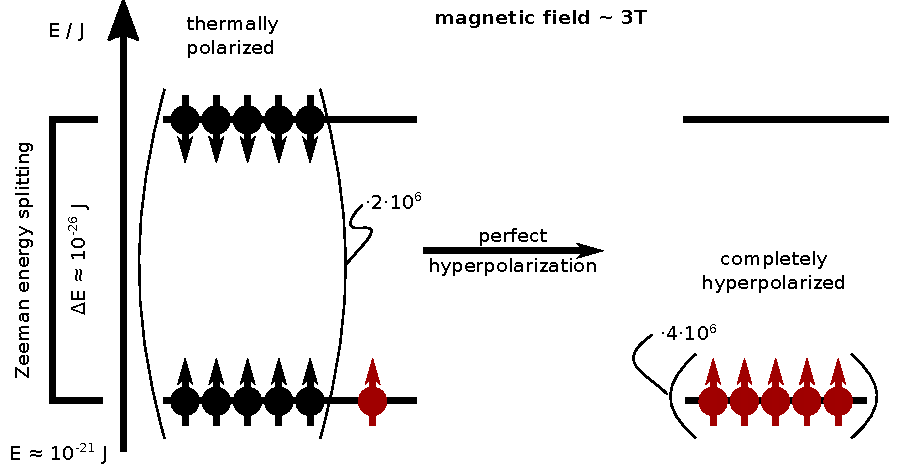
\includegraphics[width=0.99\textwidth]{/figures/theory/hyperpolarizationScheme.pdf}
            \caption[Hyperpolarization scheme]{Hyperpolarization can provide the means to drop all, or at least a lot more than in the thermally polarized case, of the spins to the lower energy level. That way, the overall magnetization and thus the signal observed is a lot higher than in ther thermally polarized case. The graph shows the case of perfect hyperpolarization, that of course does not exit in reality. At the fields currently generatable, only about one in 100000 spins effectively contributes to the signal.}
        \end{figure}
        \subsection{Dynamic nuclear polarization}
            As the gyromagnetic ratio of electrons is much higher than that of any nucleus (factor of $10^{3}$ compared to protons), dynamic nuclear polarization (DNP) uses electrons at low temperatures and high fields to generate large initial polarization. The polarization is then transferred to specific nuclei by microwave irradiation that induces transitions in the spin system of nucleus and electron that is generated by the addition of free radicals. The low temperatures lead to a freezing of the sample and microwaves are applied in that frozen state. For administration, the frozen sample then needs to be quickly melted and transferred, usually in controlled magnetic environments to prevent fast relaxation. The samples can show high polarizations close to unity but are usually limited by decay during the relatively long delivery times. Efforts building faster transport mechanisms have greatly reduced these times but they stay in the range of tens of seconds.
        \subsection{Hyperpolarization of noble gases}
            Noble gases such as 3He or 129Xe can be hyperpolarized by optical pumping. To do so, usually lasers are focused onto an optical cell through which the gas flows. Hyperpolarized gases are primarily used in lung imaging, but other uses e.g. in liquid state NMR or MRI are not precluded.
            The hyperpolarization is induced via the polarization of electron spins. An alkali metal, often Rubidium, serves as a receptor for the optical pumping and subsequently hyperpolarizes the nuclei of the noble gas by spin exchange interactions.
        \subsection{Brute force hyperpolarization}
            As equation \ref{equation:theory:polarization} indicates, there are two main factors influencing polarizatoin: Magnetic field and temperature. It is not an option to freeze the objects to be measured of course, as strong polarization effects occur only close to absolute zero temperatures at the magnetic fields we can currently generate effectively. A viable alternative is to hyperpolarize a frozen tracer at high fields, thawing it and administering it to the subject. Here, in contrast to DNP, no free radicals are necessary to generate the HP. This makes a faster and mor lossles transfer of the sample to the subject possible.
        \subsection{Parahydrogen induced Hyperpolarization}
            Parahydrogen is the singlet state of the hydrogen molecule, i.e. the antisymmetric mixed up/down state. Hydrogen molecules occur in one of the four states
            \begin{equation}
                 \begin{aligned}
                    T_+ &= |\uparrow\uparrow\rangle\\
                    T_0 &= \frac{1}{\sqrt{2}}\left(|\uparrow\downarrow\rangle + |\downarrow\uparrow\rangle\right)\\
                    T_- &= |\downarrow\downarrow\rangle\\
                    S &= \frac{1}{\sqrt{2}}\left(|\uparrow\downarrow\rangle - |\downarrow\uparrow\rangle\right)
                 \end{aligned}
            \end{equation}
            where T indicates the triplet state with overall spin I = 1 and S the singlet state with I = 0. At room temperature, the four states are almost equally occupied as thermal Energy is large compared to rotational energies of the molecule\todo{better wording}\cite{theTheoryAndPracticeOfHyperpolarizationInMrUsingh2}:
            \begin{equation}
                \frac{N_{ortho}}{N_{para}} = \frac{\sum_{J=even}(2J+1)\exp\left(-\frac{J(J+1)\Theta_R}{T}\right)}{3\sum_{J=odd}\left(2J+1\right)\exp\left(-\frac{J(J+1)\Theta_R}{T}\right)}
            \end{equation}
            which is $\tfrac{1}{3}$ plus terms depending on the ratio of thermal energy and rotational energy constant of the molecule. J is the rotational quantum number, $\Theta_R$ is the rotational energy constant of parahydrogen\cite{ortohydrogen,parahydrogenAndHeavyHydrogen}. At room temperature, the rotational energies can almost be neglected compared to thermal energy and the fraction is 1:3. Approaching absolute zero, the fraction of pH2 rises towards the pure pH2 state (see figure \ref{figure:theory:ph2Fraction}). At temperatures used to generate parahydrogen in this work, around \SI{21}{\kelvin}, the pH2 fraction is already close to 1.
            The conversion of oH2 to pH2 and back is forbidden quantum mechanically due to the change in angular momentum that would change the symmetry of the wavefunction. Therefore, conversions are only possible if different molecules collide and the nuclei interact or the rotational magnetic momentum interacts with one of the nuclei, which is both improbable and thus slow. To be able to generate pH2 in fast and in large quantities, additional interaction needs to be introduced that catalyzes the conversion. Both charcoal catalysts and ironoxide have been proposed \cite{}. The catalyst creates field gradients on the scale of the hydrogen molecule which enables spin mixing of ortho and para states\cite{spinCatalysisOfOrthoParaHydrogenConversion} and thus a much faster conversion. This means that at liquid helium temperatures which were used in this work, parahydrogen can be enriched to almost \SI{100}{\%}, a liquid nitrogen generator would enrich it to about \SI{65}{\%}.
            As parahydrogen itself is a spin 0 particle, it is MR-invisible. Its ordered state can be used though to polarize other molecules, often referred to as substrate molecules.
            \begin{figure}
                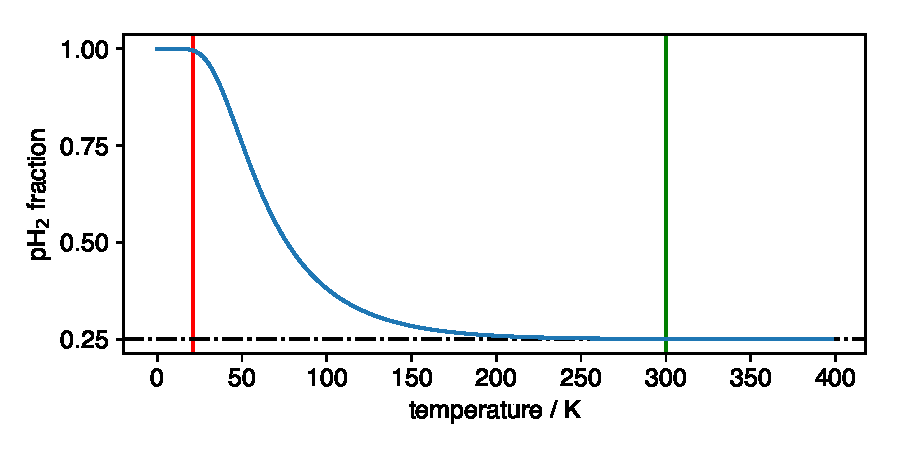
\includegraphics[width=0.99\textwidth]{/figures/theory/parahydrogenFraction.pdf}
                \caption[Parahydrogen fraction]{The equilibrium poplulation of the para hydrogen state. The dashed line shows the high temperature limit of 3:1. The green line indicates room temperature, where the limit is almost reached. The red line indicates the temperature at which parahydrogen was generated in this work, \SI{21}{\kelvin}.}
                \label{figure:theory:ph2Fraction}
            \end{figure}
        \subsubsection{Pasadena / Altadena}
        The first hyperpolarization experiments were performed at the CIT in Pasadena, and later named after it. These first experiments used parahydrogen to hydrogenate a molecule first and then used pulse sequences or field shuttling to transfer the hydrogens spin order to other nuclei. Mostly, 13C nuclei were used as recipients. of the spin order and susequent polarization. Figure \ref{} visualizes the hyperpolarization procedure. To make hyperpolarization possible, the parahydrogen needs to be added to the molecule pairwise. Furthermore, after the addition, the symmetry of the added hydrogen molecule must be broken to be able to transfer the spin order. This usually happens alredy through the asymmetry of the receptor molecule and the different couplings of each added hydrogen atom to the nuclei of the molecule.
        \subsubsection{Sabre}
        In Sabre, the molecule to be hyperpolarized is not hydrogenated, but is in contact with the parahydrogen via a catalyst for a certain contact time. The transfer of spin order can happen spontaneously at the right fields where socalled level-anti-crossings occur. In addition hyperpolarized susbtrate can also be generated at other fields using RF-irradiation. The system can be described by time evolution in bound and unbound state where the bound state implies non zero couplings between ph2 and at least some of the substrate spins.
        \begin{figure}
            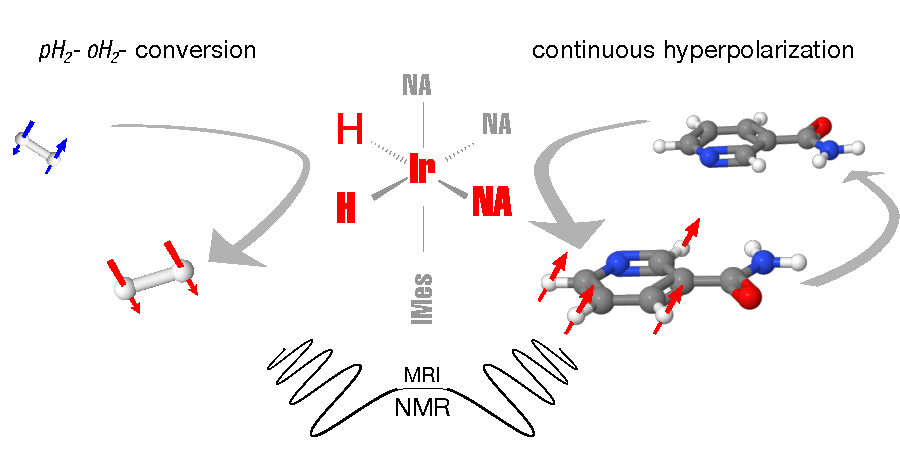
\includegraphics[width=0.99\textwidth]{/figures/theory/sabreScheme.pdf}
            \caption[Sabre scheme]{The mechanism used in Sabre using nicotinamide as an exemplary molecule. On the left, parahydrogen is converted to its ortho state, thus spin order is lost. On the right, nicotinamide is hyperpolarized using that order.}
        \end{figure}
        \section{Hardware}
            As hardware plays an important role in this work, I also want to provide some theoretical insight into some of the technologies used in this work.
            \subsection{Field generation}
                Fields are generated by either current flown conductors or superconductors. Both have ad- and disadvantages and are chosen according to requirements (see ref{methods}). Magnetic field is generated according to the fourth Maxwell equation
                \begin{equation}
                    \vec\nabla\times\vec B = \mu_0\vec j+\mu_0\epsilon_0\frac{\partial\vec E}{\partial t}
                \end{equation}
                where $\vec j$ is the electric current generating the magnetic field together with changes in the electric field. For the static field of conductor, the current is the main mechanism for field generation and is described by the Biot-Savart-law.
                \subsubsection{Normal conductors}
                A normal conductor has the great advantage of room temperature operatiion simplifying its setup and operation enormously. The disadwantage is that the conductor will heat due to its finite resistance. That heating can be so large that melting of the conductor occurs or, in the less dramatic case, deformations happen due to heat expansion. Usually copper is chosen for its low electric resistance of \SI{1.72e-8}{\ohm\meter}\ref{}(reducing heat generation) and at the same time high thermal conductivity \SI{380}{\watt\per\m\per\kelvin}\ref{DIN 4108}(increasing heat dissipation). 
                \subsubsection{Superconductors}
                Superconductors are a special form of conductors that show electric resistances of exactly zero below a certain critical temperature $T_c$. Generally, the superconductors need to be cooled from room temperature to a few \SI{}{\kelvin} to show this property, so called high temperature superconductors raised that limit to about \SI{200}{\kelvin}. Superconductors can be made of different, exotic materials but also more common substances such as graphene can show superconducting properties.Different superconductors show different critical Temperatures and mechanical properties often restricting their use to certain areas. Microscopically, inside the superconductors, so called cooper pairs are forming if the thermal energy is below \todo{finish}
            \subsection{Oscillating circuit}
            A coil usually consists of oscillatory circuits made up of a capacitor and a coil. Inside a resonsnt circuit, Energy can be stored in the form of electric field and electric current. The two forms of energy are constantly converted into each other, i.e. the capacitor is charged by the current from the coil and in turn generates a phase shifted countering current. The freuqency of this coversion can be calculated considering the following differential equations:
            \begin{equation}
                \begin{aligned}
                    -L\frac{dI}{dt} &= \frac{Q}{C} \\
                    L\frac{d^2I}{dt^2} + \frac{I}{C} &= 0
                \end{aligned}
            \end{equation}
            as the voltages of coil - that is proportional to the change in current according to Faradays law - and the capacitor - that depends on capacitance and charge - need to be equal at all times. The solution of this simplified case resulting in a ordinary second order differential equation with no linear term is simply a undampened oscillation:
            \begin{equation}
                I(t) =  A \cdot \cos(\omega t) + \phi 
            \end{equation}
            where $f= \frac{1}{\omega} = \frac{1}{2\pi\sqrt{LC}}$ which means that by changing capacitance and inductance in a resonant circuit, the resulting resonance frequency can be changed. Moreover, capacitance and inductance sizes can be adapted in opposite directions depending on the purpose of operation.
            Of course, in realistic cases, the oscillation is dampened by ohmic resistance of the components and radiation losses. 
